\documentclass{llncs}

\newcommand{\isDraft}{true}

\usepackage{amsmath}
\usepackage[usenames,dvipsnames]{color}
\usepackage{listings}
\usepackage[a4paper, top=2cm, bottom=3cm, left=2cm, right=2cm]{geometry}
\usepackage{graphicx}

\newcommand{\isDraft}{false}
\newcommand{\bfc}{{\sc Bfc}}
\newcommand{\mist}{{\sc Mist}}
\newcommand{\iic}{{\sc IIC}}
\newcommand{\pnerf}{{\sc Pnerf}}
\newcommand{\zthree}{{\sc Z3}}
\newcommand{\ttt}[1]{\texttt{#1}}

\usepackage{tikz}
\usetikzlibrary{arrows,shapes,shapes.multipart,shapes.geometric,
	snakes,automata,backgrounds,petri,calc,positioning}


\tikzstyle{place}=[circle,thick,draw=black!75,fill=white!20,
  	minimum size=6mm]
\tikzstyle{red place}=[place,draw=red!75,fill=red!20]
\tikzstyle{blue place}=[place,draw=blue!75,fill=blue!20]
\tikzstyle{transition}=[rectangle,thick,draw=black!75,
  	fill=black!20,minimum size=4mm]

\tikzstyle{state}=[draw, ellipse, aspect=2]
\tikzstyle{action}=[draw, rectangle, align=center]
\tikzstyle{decision}=[draw, diamond, aspect=2, align=center]
\tikzstyle{print}=[draw, trapezium, trapezium left angle=70, trapezium right angle=-70]
\tikzstyle{every edge}=[draw, ->, >=stealth, shorten >=2pt, shorten <=2pt]

\ifthenelse{\equal{\isDraft}{true}}{
  \usepackage[a4paper, top=2cm, bottom=3cm, left=2cm, right=2cm]{geometry}
  \pagestyle{plain}
}{}

\begin{document}

\ifthenelse{\equal{\isDraft}{false}}{
  \title{An SMT-based Approach to Coverability Analysis}
  \author{
    Javier Esparza\inst{1}
    \and
    Rupak Majumdar\inst{2}
    \and
    Philipp Meyer\inst{1}
    \and
    Filip Niksic\inst{2}
    \and
    Rusl\'{a}n Ledesma-Garza\inst{1}
  }
  \institute{
    Technische Universit\"at M\"unchen
    \and
    MPI-SWS, Kaiserslautern and Saarbr\"ucken
  }
  
  \maketitle

  \begin{abstract}
    Model checkers based on Petri net coverability have been used
    successfully in recent years to verify safety properties of concurrent
    shared-memory or asynchronous message-passing software. The bottleneck
    in the verification process is the iterative computation of the
    (backward) reachable or (forward) coverable set, and most recent
    research has focused on non-trivial heuristics to speed it up.

    In this paper, we revisit a constraint approach to the problem based on
    classical Petri net analysis techniques: marking equation, place
    invariants, and traps. Given a marking M to be covered, the approach
    constructs constraints corresponding to increasingly precise
    overapproximations of the reachable markings covering M. If one of
    these constraints is unsatisfiable, then M is not coverable.

    Previous work on this approach suffered from the absence of efficient
    decision procedures for linear arithmetic, which nowadays exist as a
    part of SMT solvers. We show how to utilize an SMT solver to implement
    the constraint approach, and additionally, to generate a minimized
    inductive invariant from a safety proof.

    We empirically evaluate our procedure on a large set of existing Petri
    net benchmarks arising out of software verification. Surprisingly, even
    though our technique is incomplete, we show that it can quickly
    discharge all safe instances, usually competitive with, and occasionally
    much faster than, state-of-the-art techniques. Additionally, the
    inductive invariants computed are usually orders of magnitude smaller
    than those produced by existing solvers.
  \end{abstract}
}{
}


\section{Introduction}

This paper makes the following contributions.
\begin{itemize}
\item An application of \zthree\ to the constraint approach and its
  corresponding evaluation.
\item A method that given a network and a property constructs a
  minimal invariant.
\end{itemize}


\section{Preliminaries}


\begin{verbatim}
* Petri net:
 N = (S, T, E, M0), where
 S : places
 T : transitions
 E : edges
 M0: initial marking

* Property:
 P, linear arithmetic formula
\end{verbatim}
\iffalse
\begin{verbatim}
 Examples:
  x + y < 0
  x + y < 0 \\and x + z > 0
  x + y < 0 \\or  x + z > 0

 ~P = (x + y <  0 \\and x + z >  0) \\or  x + z >  0
  P = (x + y >= 0 \\or  x + z <= 0) \\and x + z <= 0
\end{verbatim}
\fi

\newpage
\section{Method Safety}

The method Safety checks that a given Petri net \verb=N= never violates a property \verb=P=.
We present the method Safety by example on Lamport's 1-bit algorithm [Esparza1997].

\begin{verbatim}
* Code

Process 1:

    bit1 := false
    while true do
p1:   bit1 := true
p2:   while bit2 do skip od
p3:   <critical section>
      bit1 := false
    od

Process 2:

    bit2 := false
    while true do
q1:   bit2 := true
q2:   if bit1 then
q3:     bit2 := false
q4:     while bit1 do skip od
        goto q1
      fi
q5:   <critical section>
      bit2 := false
od

* Property: Process 1 and Process 2 are never in their respective critical section at the same time.

* Petri net:

\end{verbatim}

\begin{center}
  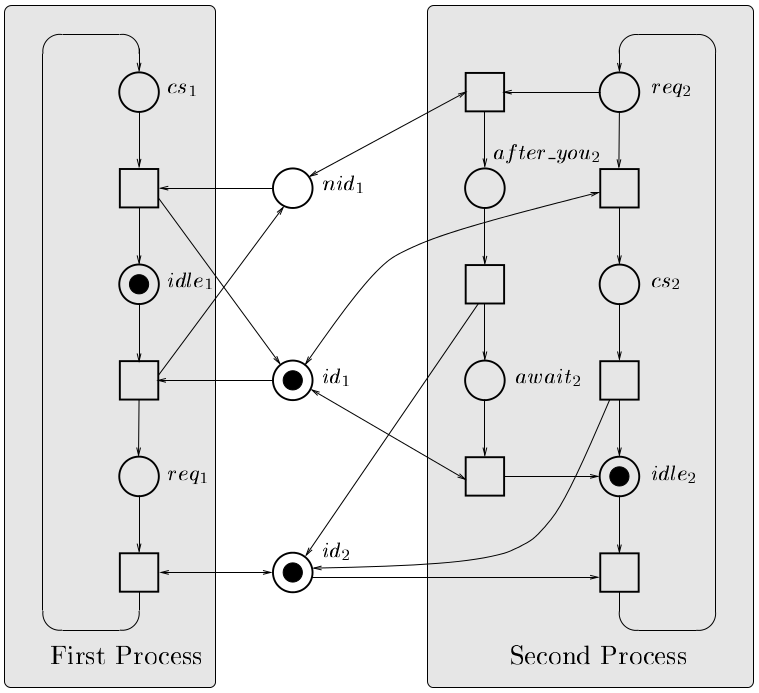
\includegraphics[width=10cm]{lamport}
\end{center}

\begin{verbatim}

* Subnet of Petri net:

\end{verbatim}

\begin{center}
\begin{tikzpicture}[node distance=1cm]
  \node[transition, label=left:t1] (t1) {};
  \node[place, tokens=1, label=left:a, below of=t1] (a) {};
  \node[transition, label=left:t2, below of=a] (t2) {};
  \node[place, tokens=0, label=left:b, below of=t2] (b) {};
  \node[place, tokens=0, label=right:$\neg bit2$, right of=t2] (nbit2) {};
  \draw (t1) edge[pre, bend left, min distance=2cm, out=225, in=-45] (b);
  \draw (t1) edge[post] (a);
  \draw (t2) edge[pre] (nbit2);
  \draw (t2) edge[post] (nbit2);
  \draw (t2) edge[pre] (a);
  \draw (t2) edge[post] (b);
\end{tikzpicture}
\end{center}

\begin{verbatim}
* Property P: a + b <= 1
\end{verbatim}

\begin{verbatim}
* Method Safety:

  Subprocedure \mathcal{C} constructs state constraints C corresponding to N.
\end{verbatim}

\begin{figure}
\begin{center}
  \begin{tikzpicture}
    \node[state] (begin) {BEGIN};
    \node[action, below=of begin] (c) {$C:=\mathcal C(N)$};
    \node[decision, below=of c] (satc) {$\text{SAT}(C \cup \{\neg P\})$};
    \node[print, right=of satc] (yes) {N satisfies P};
    \node[print, below=of satc] (dontknow) {Don't know};
    \node[state, right=of yes] (end1) {END};
    \node[state, below=of dontknow] (end2) {END};
    
    \draw (begin) edge (c);
    \draw (c) edge (satc);
    \draw (satc) edge node[above]{NO} (yes);
    \draw (yes) edge (end1);
    \draw (satc) edge node[right]{YES} (dontknow);
    \draw (dontknow) edge (end2);
  \end{tikzpicture}
\end{center}
\caption{Diagram for Method Safety}
\label{fig:method-safety-pseudocode}
\end{figure}

\begin{figure}
\begin{algorithmic}[1]
\State $C := \mathcal C(N)$
\If {SAT$(C \cup \{\neg P\})$}
  \State \Return 'The petri net may not satisfy the property'
\Else
  \State \Return 'The petri net satisfies the property!'
\EndIf
\end{algorithmic}
\caption{Pseudocode for Method Safety}
\label{fig:method-safety-pseudocode}
\end{figure}

\begin{verbatim}
* Property of state constraints C: If C U {\neg P} is unsat then N |= P.
\end{verbatim}

\newpage

\begin{verbatim}
* Example:
  - State constraints C:

    Place equations:
  
    a     = 1 + t1 - t2
    ^       ^   ^    ^
    |       |   |    |
    |       |   |    |
    |       |   |    |
    |       |   |   # of tokens taken from a
    |       |   |    
    |       |  # of tokens given to a
    |       |
    |      initial number of tokens in a
    |
    number of tokens in a

    b     = 0 - t1 + t2
    nbit2 = 0
    
Non-negativity conditions:
  
    a     >= 0
    b     >= 0
    nbit2 >= 0

  - Negated Property \neg P:

    a + b >= 2

* Place equation:
  
  For a given place s the place equation is

  # of tokens in s = initial number of tokens of place s
                     + # times each input transition of s fires
                     - # times each output transition of s fires

* Non-negativity conditions:

  # of tokens in place s           >= 0
  # of times transition t is fired >= 0

* Subprocedure \mathcal{C}:

  Input:
    (S, T, E, M0) : Petri net
  Output:
    C : State constraints

  Pseudocode:

  \end{verbatim}
\begin{align*}
  C(S, T, E, M_0) :=& \left( \bigwedge_{s \in S} \left(
    s = M_0(s) + \sum_{(t, s) \in E} t - \sum_{(s, t) \in E} t
  \right) \right) \land
    \left( \bigwedge_{s \in S} s \ge 0 \right) \land
    \left( \bigwedge_{t \in T} t \ge 0 \right)
\end{align*}

\newpage

\section{Method Safety by Refinement}

The method Safety by Refinement applies trap conditions to check that a given Petri net \verb=N= never violates a property \verb=P=.

\begin{verbatim}
* Method Safety by Refinement:

  Subprocedure TrapConditions constructs trap conditions C_\theta corresponding to N and A.
  Subprocedure \Delta constructs refinement constraint \delta corresponding to A_\theta.
\end{verbatim}

\begin{figure}
\begin{center}
\begin{tikzpicture}
  \node[state] (begin) {BEGIN};
  \node[action, below=of begin] (c) {$C:=\mathcal C(N)$};
  \node[decision, below=of c] (satc) {$\text{SAT}(C \cup \{\neg P\})$};
  \node[action, below=of satc] (modelc) {$A:=\text{Model}(C \cup \{\neg P\})$\\
                               	$C_{\theta}:=\text{TrapConditions}(N, A)$};
  \node[decision, below=of modelc] (satctheta) {$\text{SAT}(C_\theta)$};
  \node[action, below=of satctheta] (modelctheta) {$A_\theta:=\text{Model}(C_\theta)$\\
                                    	$\delta:=\Delta(A_\theta)$\\
                                    	$C:=C \cup \{\delta\}$};
  \node[print, right=of satc] (yes) {N satisfies P};
  \node[print, right=of satctheta] (dontknow) {Don't know};
  \node[state, right=of yes] (end1) {END};
  \node[state, right=of dontknow] (end2) {END};

  \draw (begin) edge (c);
  \draw (c) edge coordinate[pos=.5] (edgein) (satc);
  \draw (satc) edge node[above]{NO} (yes);
  \draw (yes) edge (end1);
  \draw (satc) edge node[right]{YES} (modelc);
  \draw (modelc) edge (satctheta);
  \draw (satctheta) edge node[above]{NO} (dontknow);
  \draw (dontknow) edge (end2);
  \draw (satctheta) edge node[right]{YES} (modelctheta);
  \draw (modelctheta.south) -- ([yshift=-0.5cm] modelctheta.south)
  -| ([xshift=-2cm] modelctheta.west) |- (edgein);
\end{tikzpicture}
\end{center}
\caption{Diagram for Method Safety by Refinement}
\label{fig:method-safety-by-refinement-diagram}
\end{figure}

\begin{figure}
\begin{algorithmic}[1]
\State $C := \mathcal C(N)$
\While {SAT$(C \cup \{\neg P\})$}
  \State $A := $Model$(C \cup \{\neg P\})$
  \State $C_\theta := $TrapConditions$(N, A)$
  \If {SAT$(C_\theta)$}
    \State $A_\theta := $Model$(C_\theta)$
    \State $\delta := \Delta(A_\theta)$
    \State $C := C \cup \{\delta\}$
  \Else
    \State \Return 'The petri net may not satisfy the property'
  \EndIf
\EndWhile
\State \Return 'The petri net satisfies the property!'
\end{algorithmic}
\caption{Pseudocode for Method Safety by Refinement}
\label{fig:method-safety-by-refinement-pseudocode}
\end{figure}

\begin{verbatim}
* Property of trap conditions C_\theta: If C_\theta is sat then there is a set S such that
  1. S is a trap in the net N
  2. S is marked in the initial marking M0
  3. S is unmarked in the assignment A

* Property of A_\theta: for each place s, A_\theta(s) iff s \in S

* Property of refinement constraint \delta: Constraint \delta refines the abstraction, i.e.
  1. A ^ \delta is unsat (\delta excludes A)
  2. N |= \delta is sat  (\delta is a property of N)
\end{verbatim}

\newpage
\begin{verbatim}
* Example
  - State constraints C same as in the example for method Safety.
 
  - Property P:

    b = 0 
  
  - Negated Property \neg P:
    
    b >= 1

  - Assignment A:
    a     = 0
    b     = 1
    nbit2 = 0
    t1    = 0
    t2    = 1

  - Trap conditions C_\theta:

    - Trap implications:
               t2
             ----------
    a     => b \/ nbit2
    ^           ^      ^
    |           |      |
    |           |     nbit2 \in S
    |           |
    |          b \in S
    |
    a \in S
    
    nbit2 => b \/ nbit2
    b     => a

    - At least one of the initially marked places belongs to S:
    a

    - None of the marked places in A belongs to S:
    ~b
  
  - Assignment A_\theta:
    a     = true
    b     = false
    nbit2 = true

  - Refinement constraint \delta:
    a + b >= 1
    ^   ^
    |   |
    -----
      |
      S = {a, b}, therefore \delta excludes assignment A in the next iteration
\end{verbatim}

\newpage

\begin{verbatim}

* Trap implication:

  place s \in S =>    /\       \    /
                     /  \       \  /     place p \in S
                    /    \       \/
                   t \in s*   p \in t*   


  "if s is in trap S then for each output transition t at least one successor p is in trap S"


* Refinement constraint \delta:

  \Sigma s >= 1  
  A(s)

  "At least one place in S is always marked"

* Subprocedure TrapConditions:

  Input:
    (S, T, E, M0) : Petri net
    A             : Satisfying assignment for C \cup { ~P }
  Output:
    C_\theta      : Trap conditions

  Pseudocode:
  
\end{verbatim}
\begin{align*}
  C_\theta(S, T, E, M_0) :=& \left( \bigwedge_{s \in S} \left( s \Rightarrow
      \bigwedge_{(s, t) \in E} \bigvee_{(t, p) \in E} p
    \right) \right) \land
    \left( \bigvee_{s \in S: M_0(s) > 0} s \right) \land
    \left( \bigwedge_{s \in S: A(s) > 0} \neg s \right)
\end{align*}
\begin{verbatim}

* Subprocedure \Delta:

  Input:
    A_\theta      : Satisfying assignment for C_\theta
  Output:
    \delta        : Refinement constraint \delta

  Pseudocode:

\end{verbatim}
\begin{align*}
  & \delta(A_\theta) := \left( \sum_{A_\theta(s)} s \ge 0 \right)
\end{align*}

\newpage
\section{Method Invariant}

The method Invariant constructs an invariant \verb=I= for given Petri net \verb=N= and \verb=P= when \verb=N= never violates \verb=P=.

\begin{verbatim}
* Code, property, and Petri net: same as in section Method Safety.
\end{verbatim}

\begin{verbatim}
* Method Invariant

  Subprocedure \mathcal{C'} constructs dual state constraints C' corresponding to N and P.
  Subprocedure Model returns assignment A such that A satisfies C'.
  Subprocedure Inv constructs invariant I corresponding to N and A'.
\end{verbatim}

\begin{figure}
\begin{center}
  \begin{tikzpicture}
    \node[state] (begin) {BEGIN};
    \node[action, below=of begin] (c) {$C':=\mathcal C'(N, \neg P)$};
    \node[decision, below=of c] (satc) {$\text{SAT}(C')$};
    \node[print, right=of satc] (noinv) {No Invariant};
    \node[action, below=of satc] (inv) {$A':=\text{Model}(C')$\\
      $I := \text{Inv}(N, A')$};
    \node[print, below=of inv] (printinv) {Invariant: $I$};
    \node[state, right=of noinv] (end1) {END};
    \node[state, below=of printinv] (end2) {END};
    
    \draw (begin) edge (c);
    \draw (c) edge (satc);
    \draw (satc) edge node[above]{NO} (noinv);
    \draw (satc) edge node[right]{YES} (inv);
    \draw (noinv) edge (end1);
    \draw (inv) edge (printinv);
    \draw (printinv) edge (end2);
  \end{tikzpicture}
\end{center}
\caption{Diagram for Method Invariant}
\label{fig:method-invariant-diagram}
\end{figure}

\begin{figure}
\begin{algorithmic}[1]
\State $C' := \mathcal C'(N, \neg P)$
\If {SAT$(C')$}
  \State $A' := $Model$(C')$
  \State $I := $Inv$(N, A')$
  \State \Return 'Invariant I for the petri net: $I$'
\Else
  \State \Return 'Failed at finding an invariant'
\EndIf
\end{algorithmic}
\caption{Pseudocode for Method Invariant}
\label{fig:method-invariant-pseudocode}
\end{figure}

\begin{verbatim}
* Property of dual state constraints C':  If C' is sat then N |= P.

* Property of invariant I:
  - I is reachable: For each reachable marking M, I(M) is valid
  - I is safe:      For markings that violate the property, I(M) is unsat
  - I is inductive: For each marking M, if I(M) is valid and M -> M1 then I(M1) is valid
\end{verbatim}

\newpage
\begin{verbatim}
* Example:

  - Dual state constraints C':

    0        >=    a  - b
    0        >= (- a) + b

    a        <  2 * target_1

    a        >= target_1
    b        >= target_1
    nbit2    >= 0
    target_1 >= 0

  - Model A':

    a        = 1
    b        = 1
    nbit2    = 1
    target_1 = 1
    
  - Invariant:

    a + b + nbit2 <= 1

\end{verbatim}

\newpage
\begin{verbatim}
* Derivation of invariant I for Petri net N that satisfies property P:

  M                                    : marking          ~ places
  C                                    : incidence matrix ~ rows correspond to places, columns correspond to transitions, relates places to transitions
  X                                    : firing vector    ~ transitions

  The following constraints C1 are unsat.
  M = M0 + C*X                         : place equations
  M >= 0                               : non-negativity conditions for places
  X >= 0                               : non-negativity conditions for transitions
  AM >= b                              : property P negated

  Substitute M to obtain constraints C2.
  A(M0 + CX) >= b                      : property P negated
  M0 + CX >= 0                         : non-negativity conditions for places
  X >= 0                               : non-negativity conditions for transitions

  Rewrite each system to obtain constraints C3.
  (-A*C)      (A*M0-b)                 : property P negated
  (  -C)*X <= (  M0  )                 : non-negativity conditions for places
  (  -I)      (   0  )                 : non-negativity conditions for transitions

  Apply Farkas' Lemma to obtain constraints C4.
  yT*(-A*C)                            : 
     (  -C) = 0                        : 
     (  -I)                            : 

  yT*(A*M0-b)                          : 
     (  M0  ) < 0                      : 
     (   0  )                          : 

  y >= 0                               : 

  The constraints C4 are sat iff the following constraints C5 are sat.
  y1 * A * C + y2 * C + y3 = 0         : 
  y1 * (A*M - b) + y2 * M0 < 0         : 
  y1 >= 0                              : 
  y2 >= 0                              : 
  y3 >= 0                              : 

  The constraints C5 are sat iff the following constraints C6 are sat.
  (y1 * A + y2) * C  <= 0              : 
  (y1 * A + y2) * M0 < y1 * b          : 
  y1 >= 0                              : 
  y2 >= 0                              : 

  The constraints C6 are sat iff the following constraints C' are sat.
  \lambda * C  <= 0                    : inductivity constraint
  \lambda * M0 < y1 * b                : safety constraint
  \lambda >= y1 * A                    : property constraint
  y1 >= 0                              : non-negativity constraint

  For \lambda satisfying C' the invariant is the following.
  I(M) = (\lambda * M <= \lambda * M0) : invariant
\end{verbatim}

\newpage
\begin{verbatim}
* Subprocedure \mathcal{C'}:

  Input:
    N = (S, T, E, M0)  : Petri net
    \neg P = (p_1,1 + ... + p_1,m_1 >= b_1 /\ p_2,1 + ... + p_2,m_2 >= b_2 /\
              ... /\ p_n,1 + ... + p_n,m_n >= b_n ) : Negated property
  Output:
    C'            : Dual state constraints

Input:
 N      = (S, T, E, M0)
        = ( (a b nbit2 ) (t1 t2) (e1 ... en) (1 0 0) )
\neg P  = ( a + b >= 2 )

Pseudocode:
\end{verbatim}

\begin{align*}
  C'(N, \neg P) =& \left( \bigwedge_{t \in T} \left( 0 \ge
                      \sum_{(t, s) \in E} s
                    - \sum_{(s, t) \in E} s \right) \right) \land
     \left( \sum_{s \in S} M_0(s) \cdot s <
       \sum_{i=1}^n b_i \cdot target_i \right) \land \\
     & \left( \bigwedge_{s \in S} \left ( s \ge 
       \sum_{i : s \in \{ p_{i,1}, \ldots, p_{i,m_i} \} } target_i \right) \right) \land
     \left( \bigwedge_{i=1}^n \left( target_i \ge 0 \right) \right)
\end{align*}

\begin{verbatim}
* Subprocedure Inv:

  Input:
    N = (S, T, E, M0) : Petri net
    A'                : Satisfying assignment for C'

  Output:
    I                 : Invariant

  Pseudocode:
\end{verbatim}

\begin{align*}
  I(N, A') =& \left( \sum_{s \in S} A'(s) \cdot s \le
                     \sum_{s \in S} A'(s) \cdot M_0(s) \right)
\end{align*}

\newpage
\section{Method Invariant with Minimization}

The method Invariant with Minimization constructs an invariant \verb=I=
that uses a minimal number of places for given Petri net \verb=N= and
\verb=P= when \verb=N= never violates \verb=P=. 

\begin{verbatim}
* Code, property, and Petri net: same as in section Method Safety.

* Method Invariant with Minimization

  Subprocedure \text{MinConstraints} constructs minimization constraints C_M corresponding to N and A'
\end{verbatim}

\begin{figure}
\begin{center}
  \begin{tikzpicture}
    \node[state] (begin) {BEGIN};
    \node[action, below=of begin] (c) {$C':=\mathcal C'(N, \neg P)$};
    \node[decision, below=of c] (satc) {$\text{SAT}(C')$};
    \node[print, right=of satc] (noinv) {No Invariant};
    \node[action, below=of satc] (model1) {$A':=\text{Model}(C')$};
    \node[action, below=of model1] (cm) {$C_M:=\text{MinConstraints}(N, A')$};
    \node[decision, below=of cm] (satcm) {$\text{SAT}(C' \cup C_M)$};
    \node[action, right=of satcm] (model2) {$A':=\text{Model}(C' \cup C_M)$};
    \node[action, below=of satcm] (inv) {$I := \text{Inv}(N, A')$};
    \node[print, below=of inv] (printinv) {Invariant: $I$};
    \node[state, right=of noinv] (end1) {END};
    \node[state, below=of printinv] (end2) {END};
    
    \draw (begin) edge (c);
    \draw (c) edge (satc);
    \draw (satc) edge node[above]{NO} (noinv);
    \draw (noinv) edge (end1);
    \draw (satc) edge node[right]{YES} (model1);
    \draw (model1) edge coordinate[pos=.5] (edgein) (cm);
    \draw (cm) edge (satcm);
    \draw (satcm) edge node[above]{YES} (model2);
    \draw (model2) |- (edgein);
    \draw (satcm) edge node[right]{NO} (inv);
    \draw (inv) edge (printinv);
    \draw (printinv) edge (end2);
  \end{tikzpicture}
\end{center}
\caption{Diagram for Method Invariant with Minimization}
\label{fig:method-invariant-with-minimization-diagram}
\end{figure}

\begin{figure}
\begin{algorithmic}[1]
\State $C' := \mathcal C'(N, \neg P)$
\If {SAT$(C')$}
  \State $A' := $Model$(C')$
  \State $C_M := $MinConstraints$(N, A')$
  \While {SAT$(C' \cup C_M)$}
    \State $A' := $Model$(C' \cup C_M)$
    \State $C_M := $MinConstraints$(N, A')$
  \EndWhile
  \State $I := $Inv$(N, A')$
  \State \Return 'Invariant I for the petri net: $I$'
\Else
  \State \Return 'Failed at finding an invariant'
\EndIf
\end{algorithmic}
\caption{Pseudocode for Method Invariant with Minimization}
\label{fig:method-invariant-with-minimization-pseudocode}
\end{figure}

\begin{verbatim}
* Property of minimization constraints C_M generated from A': 
    If A'' satisfies C' u C_M, then Inv(N, A'') uses less places than Inv(N, A')
\end{verbatim}

\newpage
\begin{verbatim}
* Example:
  - Dual state constraints C' and satisfying assignment A' for C' as in example for method Invariant

  - Minimization constraints C_M:

    a     > 0 => b_a     = 1
    |            -----------
    |               |
    |            place appears in invariant
    |
    place coefficient in the invariant

    a     = 0 => b_a     = 0
    |           ------------
    |               |
    |            place does not appear in invariant
    |
    place coefficient in the invariant

    b     > 0 => b_b     = 1
    b     = 0 => b_b     = 0
    nbit2 > 0 => b_nbit2 = 1
    nbit2 = 0 => b_nbit2 = 0

    b_a + b_b + b_nbit2 < 3
    -------------------   |
                |         |
                |    number of places appearing in current invariant for A'
                |    = #{s | A'(s) > 0} = #{a, b, nbit2}
                |
  number of places appearing in new invariant
  
  - Model A' for C' \cup C_M:

    a        = 1
    b        = 1
    nbit2    = 0
    target_1 = 1
    
  - Minimized Invariant:

    a + b <= 1
    
* Subprocedures \mathcal{C'} and Inv are the same as
  in Method Invariant

* Subprocedure \text{MinConstraints}:

  Input:
    N = (S, T, E, M0)  : Petri net
    A'                 : Satisfying assignment for C'
  Output:
    C_M                : Minimization Constraints

  Pseudocode:

\end{verbatim}

\begin{align*}
  C_M(N, A') =& \left( \bigwedge_{s \in S} \left(
      (s > 0 \Rightarrow b_s = 1) \land (s = 0 \Rightarrow b_s = 0)
    \right) \right) \land
    \left( \sum_{s \in S} b_s < \sum_{s \in S : A'(s) > 0} 1 \right)
\end{align*}

\newpage

\section{Method Invariant by Refinement}

\begin{verbatim}
* Code, property, and Petri net: same as in section Method Safety by Refinement.

* Method Invariant by Refinement
\end{verbatim}

\begin{figure}
\begin{tikzpicture}
  \node[state] (begin) {BEGIN};
  \node[action, below=of begin] (c) {$C:=\mathcal C(N)$\\
                                        $D:=\{\}$};
  \node[decision, below=of c] (satc) {$\text{SAT}(C \cup \{\neg P\})$};
  \node[action, below=of satc] (modelc) {$A:=\text{Model}(C \cup \{\neg P\})$\\
                                        $C_{\theta}:=\text{TrapConditions}(N, A)$};
  \node[decision, below=of modelc] (satctheta) {$\text{SAT}(C_\theta)$};
  \node[action, below=of satctheta] (modelctheta) {$A_\theta:=\text{Model}(C_\theta)$\\
                                                $\delta:=\Delta(A_\theta)$\\
                                                $C:=C \cup \{\delta\}$\\
                                                $D:=D \cup \{\delta\}$};
  \node[print, right=of satctheta] (noinv2) {No Invariant};
  \node[state, below=of noinv2] (end3) {END};
   
  \node[action, right=of satc] (cprime) {$C':=\mathcal C'(N, \neg P \land D)$};
  \node[decision, right=of cprime] (satcprime) {$\text{SAT}(C')$};
  \node[action, below=of satcprime] (inv) {$A':=\text{Model}(C')$\\
                                        $I:=D \land \text{Inv}(N, A')$};
  \node[print, below=of inv] (printinv) {Invariant: $I$};
  \node[print, right=of satcprime] (noinv) {No Invariant};
  \node[state, below=of noinv] (end1) {END};
  \node[state, below=of printinv] (end2) {END};
 
  \draw (cprime) edge (satcprime);
  \draw (satcprime) edge node[above]{NO} (noinv);
  \draw (satcprime) edge node[right]{YES} (inv);
  \draw (inv) edge (printinv);
  \draw (noinv) edge (end1);
  \draw (printinv) edge (end2);
 
  \draw (begin) edge (c);
  \draw (c) edge coordinate[pos=.5] (edgein) (satc);
  \draw (satc) edge node[above]{NO} (cprime);
  \draw (satc) edge node[right]{YES} (modelc);
  \draw (modelc) edge (satctheta);
  \draw (satctheta) edge node[above]{NO} (noinv2);
  \draw (noinv2) edge (end3);
  \draw (satctheta) edge node[right]{YES} (modelctheta);
  \draw (modelctheta.south) -- ([yshift=-0.5cm] modelctheta.south)
  -| ([xshift=-2cm] modelctheta.west) |- (edgein);
\end{tikzpicture}
\caption{Diagram for Method Invariant by Refinement}
\label{fig:method-invariant-by-refinement-diagram}
\end{figure}

\begin{figure}
\begin{algorithmic}[1]
\State $C := \mathcal C(N)$
\State $D := $true
\While {SAT$(C \cup \{\neg P\})$}
  \State $A := $Model$(C \cup \{\neg P\})$
  \State $C_\theta := $TrapConditions$(N, A)$
  \If {SAT$(C_\theta)$}
    \State $A_\theta := $Model$(C_\theta)$
    \State $\delta := \Delta(A_\theta)$
    \State $C := C \cup \{\delta\}$
    \State $D := D \land \delta$
  \Else
    \State \Return 'Failed at finding an invariant'
  \EndIf
\EndWhile
\State $C' := \mathcal C'(N, \neg P \land D)$
\If {SAT$(C')$}
  \State $I := D \land $Inv$(N, A')$
  \State \Return 'Invariant I for the petri net: $I$'
\Else
  \State \Return 'Failed at finding an invariant'
\EndIf
\end{algorithmic}
\caption{Pseudocode for Method Invariant by Refinement}
\label{fig:method-invariant-by-refinement-pseudocode}
\end{figure}

\newpage

\begin{verbatim}
* Example:

  - Trap constraints as in example from section Method Safety by Refinement.
  
  - Dual state constraints C':

    0        >=    a  - b
    0        >= (- a) + b

    a        <  target_1 + trap_1

    a        >= trap_1
    b        >= target_1
    nbit2    >= trap_1
    target_1 >= 0
    trap_1   >= 0

  - Model A':

    a        = 1
    b        = 1
    nbit2    = 1
    target_1 = 1
    trap_1   = 1
    
  - Invariant:

    a     + nbit2 >= 1
    a + b + nbit2 <= 1

* Subprocedures TrapConditions and \Delta are the same as
  in Method Safety by Refinement

* Subprocedures \mathcal{C'} and Inv are the same as
  in Method Invariant
\end{verbatim}

\iffalse

\newpage
\section{Benchmarks of \bfc}

We experimented on the benchmarks \ttt{cprover-PN} and
\ttt{cprover\_software\_analysis} available at \\
\ttt{http://www.mpi-sws.org/\~{}jkloos/iic-experiments/cprover.zip}.
The set of benchmarks consists 77 benchmarks, 26 positive and 51 negative.
Table~\ref{bfc-experiments} shows the corresponding experimental results.

\begin{table}[h]
\begin{center}
  \begin{tabular}{ | p{7cm} | r | r | r | r | } %
    \hline
    Method & pos & neg & don't know & TO \\
    \hline
    Safety (over real numbers or naturals)      & 23 &  0 & 54 &  0 \\
    Invariant \& Invariant with Minimization    & 23 &  0 & 54 &  0 \\
    Safety by Refinement                        & 23 &  0 & 54 &  0 \\
    \hline
  \end{tabular}
\end{center}
\caption{Experimental results for the benchmarks of \bfc}
\label{bfc-experiments}
\end{table}

\section{Benchmarks of \mist}

We experimented on the benchmarks available at \\
\ttt{https://github.com/pierreganty/mist/tree/master/examples/boundedPN}
and \\
\ttt{https://github.com/pierreganty/mist/tree/master/examples/PN}.
The set of benchmarks consists 27 benchmarks, 23 positive and 4 negative.
Table~\ref{mist-experiments} shows the corresponding experimental results.

\begin{table}[h]
\begin{center}
  \begin{tabular}{ | p{6cm} | r | r | r | r | }
    \hline
    Method & pos & neg & don't know & TO \\
    \hline
    Safety (over real numbers or naturals)      & 14 &  0 & 13 &  0 \\
    Invariant \& Invariant with Minimization    & 14 &  0 & 13 &  0 \\
    Safety by Refinement                        & 20 &  0 &  7 &  0 \\
    \hline
  \end{tabular}
\end{center}
\caption{Experimental results for the benchmarks of \mist}
\label{mist-experiments}
\end{table}

\section{Benchmarks of \iic}

We experimented on the benchmarks available at \\
\ttt{https://svn.rse.mpi-sws.org/RSE/IC3forWSTS/code/trunk/examples/soter}.
The set of benchmarks consists 38 benchmarks, 28 positive and 10 negative.
Table~\ref{iic-experiments} shows the corresponding experimental results.

\begin{table}[h]
\begin{center}
  \begin{tabular}{ | p{6cm} | r | r | r | r | }
    \hline
    Method & pos & neg & don't know & TO \\
    \hline
    Safety (over real numbers or naturals)      & 2 & 0 & 36 & 0 \\
    Invariant \& Invariant with Minimization    & 2 & 0 & 26 & 0 \\
    Safety by Refinement                        & 2 & 0 & 36 & 0 \\
    \hline
  \end{tabular}
\end{center}
\caption{Experimental results for the benchmarks of \iic}
\label{iic-experiments}
\end{table}

We constructed the following two invariants by applying the method
Invariant with Minimization.

\begin{itemize}
\item \verb?firewall__no_pred_called_with_zero__depth_1__fixed?: \verb?(assert (<= l739 0))?
\item \verb?firewall__no_pred_called_with_zero__depth_2__fixed?: \verb?(assert (<= l3849 0))?
\end{itemize}

\iic\ constructs the following two invariants.

\begin{itemize}
\item \verb=firewall__no_pred_called_with_zero__depth_1__fixed.spec=: \verb=(l739 < 1)=
\item \verb=firewall__no_pred_called_with_zero__depth_2__fixed.spec=: \verb=(l3849 < 1)=
\end{itemize}

\fi

\end{document}
